%File: formatting-instructions-latex-2024.tex
%release 2024.0
\documentclass[letterpaper]{article} % DO NOT CHANGE THIS
\usepackage{aaai24}  % DO NOT CHANGE THIS
\usepackage{times}  % DO NOT CHANGE THIS
\usepackage{helvet}  % DO NOT CHANGE THIS
\usepackage{courier}  % DO NOT CHANGE THIS
\usepackage[hyphens]{url}  % DO NOT CHANGE THIS
\usepackage{graphicx} % DO NOT CHANGE THIS
\usepackage[T1]{fontenc}
\urlstyle{rm} % DO NOT CHANGE THIS
\def\UrlFont{\rm}  % DO NOT CHANGE THIS
\usepackage{natbib}  % DO NOT CHANGE THIS AND DO NOT ADD ANY OPTIONS TO IT
\usepackage{caption} % DO NOT CHANGE THIS AND DO NOT ADD ANY OPTIONS TO IT
\frenchspacing  % DO NOT CHANGE THIS
\setlength{\pdfpagewidth}{8.5in}  % DO NOT CHANGE THIS
\setlength{\pdfpageheight}{11in}  % DO NOT CHANGE THIS
%
% These are recommended to typeset algorithms but not required. See the subsubsection on algorithms. Remove them if you don't have algorithms in your paper.
\usepackage{algorithm}
\usepackage{algorithmic}

%
% These are are recommended to typeset listings but not required. See the subsubsection on listing. Remove this block if you don't have listings in your paper.
\usepackage{newfloat}
\usepackage{listings}
\DeclareCaptionStyle{ruled}{labelfont=normalfont,labelsep=colon,strut=off} % DO NOT CHANGE THIS
\lstset{%
    basicstyle={\footnotesize\ttfamily},% footnotesize acceptable for monospace
    numbers=left,numberstyle=\footnotesize,xleftmargin=2em,% show line numbers, remove this entire line if you don't want the numbers.
    aboveskip=0pt,belowskip=0pt,%
    showstringspaces=false,tabsize=2,breaklines=true}
\floatstyle{ruled}
\newfloat{listing}{tb}{lst}{}
\floatname{listing}{Listing}
%
% Keep the \pdfinfo as shown here. There's no need
% for you to add the /Title and /Author tags.
\pdfinfo{
/TemplateVersion (2024.1)
}

\graphicspath{ {./assets/} }

% DISALLOWED PACKAGES
% \usepackage{authblk} -- This package is specifically forbidden
% \usepackage{balance} -- This package is specifically forbidden
% \usepackage{color (if used in text)
% \usepackage{CJK} -- This package is specifically forbidden
% \usepackage{float} -- This package is specifically forbidden
% \usepackage{flushend} -- This package is specifically forbidden
% \usepackage{fontenc} -- This package is specifically forbidden
% \usepackage{fullpage} -- This package is specifically forbidden
% \usepackage{geometry} -- This package is specifically forbidden
% \usepackage{grffile} -- This package is specifically forbidden
% \usepackage{hyperref} -- This package is specifically forbidden
% \usepackage{navigator} -- This package is specifically forbidden
% (or any other package that embeds links such as navigator or hyperref)
% \indentfirst} -- This package is specifically forbidden
% \layout} -- This package is specifically forbidden
% \multicol} -- This package is specifically forbidden
% \nameref} -- This package is specifically forbidden
% \usepackage{savetrees} -- This package is specifically forbidden
% \usepackage{setspace} -- This package is specifically forbidden
% \usepackage{stfloats} -- This package is specifically forbidden
% \usepackage{tabu} -- This package is specifically forbidden
% \usepackage{titlesec} -- This package is specifically forbidden
% \usepackage{tocbibind} -- This package is specifically forbidden
% \usepackage{ulem} -- This package is specifically forbidden
% \usepackage{wrapfig} -- This package is specifically forbidden
% DISALLOWED COMMANDS
% \nocopyright -- Your paper will not be published if you use this command
% \addtolength -- This command may not be used
% \balance -- This command may not be used
% \baselinestretch -- Your paper will not be published if you use this command
% \clearpage -- No page breaks of any kind may be used for the final version of your paper
% \columnsep -- This command may not be used
% \newpage -- No page breaks of any kind may be used for the final version of your paper
% \pagebreak -- No page breaks of any kind may be used for the final version of your paperr
% \pagestyle -- This command may not be used
% \tiny -- This is not an acceptable font size.
% \vspace{- -- No negative value may be used in proximity of a caption, figure, table, section, subsection, subsubsection, or reference
% \vskip{- -- No negative value may be used to alter spacing above or below a caption, figure, table, section, subsection, subsubsection, or reference

\setcounter{secnumdepth}{0} %May be changed to 1 or 2 if section numbers are desired.

% The file aaai24.sty is the style file for AAAI Press
% proceedings, working notes, and technical reports.
%

% Title

% Your title must be in mixed case, not sentence case.
\title{Hierarchical Reinforcement Learning: Maze with Tasks}
\author {
    % Authors
    Rubén Cid Costa\textsuperscript{\rm 1},
    Aimar Nicuera Usandizaga\textsuperscript{\rm 2},
    Daniel Obreo Sanz\textsuperscript{\rm 3}
}
\affiliations {
    % Affiliations
    \textsuperscript{\rm 1, \rm 2, \rm 3}Universidad Carlos III de Madrid\\
    
    \textsuperscript{\rm 1}100538592@alumnos.uc3m.es, 
    \textsuperscript{\rm 2}100537352@alumnos.uc3m.es, 
    \textsuperscript{\rm 3}100451058@alumnos.uc3m.es 
}

% REMOVE THIS: bibentry
% This is only needed to show inline citations in the guidelines document. You should not need it and can safely delete it.
\usepackage{bibentry}
% END REMOVE bibentry

\begin{document}

\maketitle

\begin{abstract}
La realización de objetivos secuenciales en un entorno es una tarea compleja de modelar y aprender. Para poder representar estos
escenarios, una de las técnicas más usadas es el Aprendizaje por Refuerzo Jerárquico (\textit{Hierarchical Reinforcement Learning (HRL)}).
En este contexto, este trabajo se enfoca en Feudal Learning, una variante de HRL que organiza las tareas en una estructura jerárquica de
niveles de abstracción. Este documento detallará las bases teóricas y su aplicación sobre un ambiente de desarrollo con tareas de navegación y
obtención de subobjetivos.
\end{abstract}

\section{Introducción}

En muchos dominios, como la robótica o sistemas autónomos, las tareas implican la realización de objetivos secuenciales en entornos complejos.
La capacidad de modelar y aprender estos escenarios es un desafío crucial para la inteligencia artificial.

El aprendizaje por refuerzo jerárquico (HRL) se presenta como un enfoque para la resolución de estos problemas. Mientras que otras técnicas previas
enfrentan dificultades para escalar con el número de tareas y su complejidad, el Aprendizaje por Refuerzo Jerárquico (HRL) organiza el proceso en 
niveles de abstracción. Dentro de este marco, el Aprendizaje Feudal se presenta como un enfoque que permite modelar las tareas mediante una jerarquía
de abstracción.

Este trabajo se centra en el estudio de Feudal Learning, una variante de HRL. Se presentan las bases teóricas de esta técnica como diferentes algoritmos
o métodos de aprendizaje que se han desarrollado en este campo. También, se mostrará su aplicación sobre un entorno simulado diseñado para tareas 
de navegación en laberintos y obtención de subobjetivos. 

\section{Marco Teórico y Estado del Arte}
% Que es el aprendizaje jerárquico
El aprendizaje por refuerzo jerárquico (HRL por sus siglas en inglés) se ha consolidado como una estrategia para abordar problemas complejos
que involucran secuencias de tareas. Este enfoque se originó como una extensión de los modelos de decisión de Markov para tareas de largo horizonte
de decisión mediante el uso de modelos semi-MDP \cite{sutton1999between}. Con ellos, se establecen las bases teóricas para la abstracción temporal.

Posteriormente, con los años, han surgido una serie de algoritmos que implementan y abordan las limitaciones de HRL. 
Dietterich \cite{dietterich2000hierarchical} propuso el modelo MaxQ, que descompone las tareas en jerarquías de subtareas
para la optimización y planificación de diferentes funciones de valor. Por otro lado, en \cite{barto2003recent} se exploran 
los avances en estructuras jerárquicas para diferentes dominios y la relevancia de HRL para la resolución de problemas de 
gran complejidad.  

% Qué el aprendizaje feudal
Dentro de este marco teórico, el Aprendizaje Feudal se presenta como una técnica que organiza las tareas en niveles jerárquicos, donde cada nivel 
es operado con distintos grados de abstracción tanto en el estado como en temporalidad. Este enfoque \cite{dayan1992feudal} divide la jerarquía en managers, que operan con abstracciones 
del estado y dan órdenes de acción y en workers que realizan las acciones. Esta colaboración jerárquica permite aprender y ejecutar tareas de manera más eficiente, aprovechando
la modularidad y la capacidad de escalar a problemas complejos.

% FuN
Otro enfoque es el propuesto por A. S. Vezhnevets et al. \cite{vezhnevets2017feudal}, que plantea las redes feudales como una arquitectura de aprendizaje por refuerzo jerárquico.
Este sistema emplea la estructura manager-worker mencionada anteriormente, pero añade redes neuronales recurrentes (específicamente LSTMs) como mecanismo de funcionamiento tanto del 
manager como del worker. Este enfoque se ha mostrado efectivo en la resolución de problemas complejos; por lo que puede ser de utilidad en la resolución del problema propuesto en este trabajo.

\subsection{Sistemas de Control Feudal}
% Que son
En 1992, P. Dayan y G. Hinton \cite{dayan1992feudal} definen los sistemas de control feudal como un reflejo de las sociedades feudales. En ellos, se 
define una jerarquía de \textit{managers}, \textit{supermanagers} y \textit{workers}. Cada uno opera con un grado de abstracción de estados y temporal
distinto. Los managers tienen poder absoluto sobre sus subordinados. Pueden dar órdenes que deben ser seguidas, dan tareas, recompensas y castigos si 
las órdenes no son seguidas. Esta estructura jerárquica de mando permite aprender y comprender tareas complejas con el fin de maximizar el refuerzo.

Este sistema de control se basa en dos principios:
\begin{itemize}
    \item \textbf{Ocultamiento de la Recompensa (Reward Hiding)}. Los \textit{managers} recompensan a los \textit{submanagers} únicamente si operan 
    en consonancia con las órdenes dadas. Los \textit{submanagers} deben aprender a obedecer y aprender que debe hacer el siguiente agente para 
    cumplir de manera eficiente. De la misma manera, el \textit{submanager} es recompensado si su subordinado ejecuta las órdenes a pesar de no llegar a cumplir 
    las ordenes propias del \textit{submanager}.

    \item \textbf{Ocultamiento de la Información (Information Hiding)}. Los \textit{managers} solamente deben conocer la información necesaria 
    con un nivel de granularidad distinto a la de los \textit{workers}. Las decisiones se toman en base a un espacio de estados menor pero más
    denso en información. También, las órdenes dadas a un \textit{submanager} no son propagadas hacia el resto de los niveles para no afectar la toma
    de decisiones. Tampoco, se propagan hacia arriba las acciones del \textit{worker} hacia el resto de los \textit{managers}. 
\end{itemize}

Estos principios siguen una dinámica de poder y gestión similar a la de sociedades feudales con diferente interés en cada estamento de la organización.
No obstante, todos se alinean para la obtención y maximización de una recompensa (o refuerzo) dado por el problema.

Para el aprendizaje e implementación, se propuso el uso de una versión modificada del Aprendizaje Q-Learning. Cada \textit{mánager}, \textit{submanager} y
\textit{worker} tiene asociada una función acción-valor (\textit{Q Tabla}). La principal diferencia con respecto al algoritmo original es la 
modificación de la función de recompensa. En este caso, se modifica en función de las acciones tomadas por cada nivel de la jerarquía en consonancia 
con su nivel de obediencia. 

\subsection{FeUdal Networks: FuN}

Las redes feudales se basan en la arquitectura de aprendizaje por refuerzo feudal \cite{vezhnevets2017feudal}, 
una arquitectura del aprendizaje por refuerzo jerárquico. Esta arquitectura emplea un sistema de control, conocido
como \textit{mánager}, que asigna tareas a un subsistema conocido como \textit{worker} que debe aprender a ejecutarlas de manera óptima.

La arquitectura del sistema se muestra en la imagen siguiente\cite{feudal_networks_2024}.

\begin{figure}[H]
    \centering
    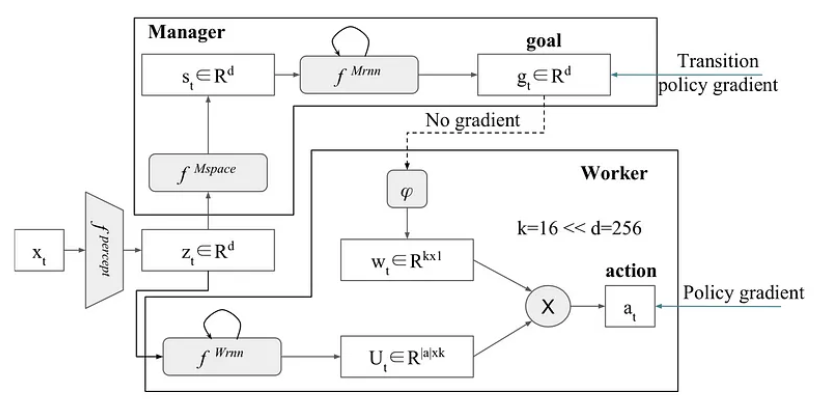
\includegraphics[width=0.9\columnwidth]{feudal_arquitecture.png}
    \caption{Arquitectura de una red feudal.\label{fig:arquitectura_feudal}}
\end{figure}

La entrada de esta red es procesada por una capa de percepción, que emplea capas convolucionales
para extraer características de la imagen de entrada. A continuación, estas características son procesadas
tanto por el worker como por el mánager, cada uno de manera distinta; el mánager extrae objetivos y el worker
aprende a alcanzar esos objetivos.

El objetivo principal del mánager es generar metas que el worker debe cumplir. Recibe la percepción
del entorno, proporcionada por el módulo de percepción, ese estado es procesado por una red recurrente LSTM
para mantener un estado interno y poder capturar información relevante en horizontes temporales largos.
El mánager emplea esta información para predecir un objetivo direccional en el espacio latente, este objetivo
es un vector unitario, lo que asegura que el worker se enfoque en la dirección y no en la posición absoluta.

Para entrenar el mánager, se emplea la recompensa obtenida, y emplea la similitud coseno entre la dirección en la que 
se movió el worker y la compara con el objetivo establecido, empleando la similitud coseno como función de pérdida.
Esta pérdida incentiva al manager a emitir objetivos que maximicen el progreso hacia estados ventajosos.

El vector de objetivos se envía al worker sin propagar gradientes, esto garantiza que los objetivos 
mantengan un significado semántico independiente, en lugar de ser simples variables latentes optimizadas de manera conjunta.

En el caso del worker, también se emplea una red LSTM para mantener un estado interno y poder capturar información relevante,
pero en este caso, el worker recibe tanto la percepción del entorno como el objetivo del mánager. El worker emplea esta información
para predecir la acción que debe realizar para alcanzar el objetivo. La acción se predice en el espacio de acciones, y se ejecuta,
lo que proporciona un nuevo estado y un refuerzo que se emplea para entrenar las redes.

\section{Evaluación práctica}
\subsection{Descripción del Experimento}

Para la realización de pruebas, se ha planteado el problema de navegación en un conjunto de laberintos. 
En cada uno de ellos, el agente tiene como tarea secundaria (obligatoria) la obtención de un conjunto de 
monedas (\textit{tokens}) para poder abrir la meta. Estas monedas están repartidas alrededor del mapa.

\begin{figure}[H]
    \centering
    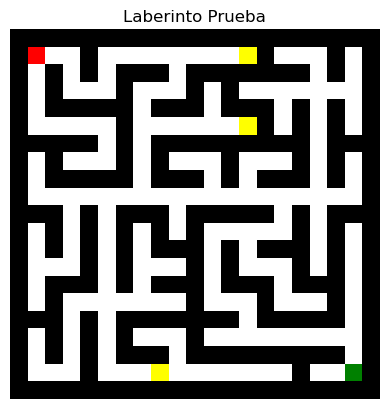
\includegraphics[width=0.7\columnwidth]{maze.png}
    \caption{Ejemplo de Laberinto con 3 monedas (cuadrado amarillo) y una meta (cuadrado verde)\label{fig:maze-example}}
\end{figure}

En términos de implementación, los laberintos se han creado usando el algoritmo de Wilson. Las monedas se posicionan
aleatoriamente en casillas libres del mapa. Para poder ser usados en CNN y RNN, por cada celda original se obtienen 4 celdas con las paredes.
Esto genera un laberinto con el doble del tamaño original, como se ve en Fig. \ref{fig:maze-example}.

Para los experimentos, se iniciaba con 0 monedas y, en base a la capacidad de aprender el camino y obtener los resultados, se añadían monedas o se cambiaba el experimento.
De esta manera, se podía estudiar de manera directa el efecto del incremento en la complejidad en la capacidad de adaptarse y aprender el laberinto. 

Se debe destacar que, en cada experimento, el laberinto generado es distinto. No se ha podido mantener el mismo laberinto en todas las ocasiones. No obstante,
se pueden comparar los resultados debido a que todos comparten las mismas características y son válidos.

Para la experimentación, los agentes tienen como estado base (previo a transformaciones propias del método) la vista global del laberinto y la posición como coordenadas. 
Como acciones base, los agentes tienen las acciones de movimiento cardinales estándar NSWE (North-South-West-East). En algunos métodos, 
también se añade la acción $*$ para los \textit{managers}.

Finalmente, aunque inicialmente se partió de episodios partiendo del punto más alejado a la meta, se decidió implementar una política de inicio aleatorio en favor de la exploración y capacidad del agente para solventar el problema desde diferentes áreas del laberinto.

\subsection{Experimento: Feudal Q-Learning}
Para comprobar la efectividad de estos métodos, se han realizado diferentes pruebas e implementaciones. El primer experimento
se basa en una implementación que refleja fielmente los alineamientos de los sistemas de control feudales descritos. 

Basándose en el ejemplo de la publicación, se han planteado una jerarquía de cuatro niveles en la que cada mánager tiene la mitad de resolución 
que el nivel anterior (Véase Fig.\ref{fig:feudal-abstract}). Además, los manager tienen acceso al estado con la presencia de monedas en cada región.  

\begin{figure}[H]
    \centering
    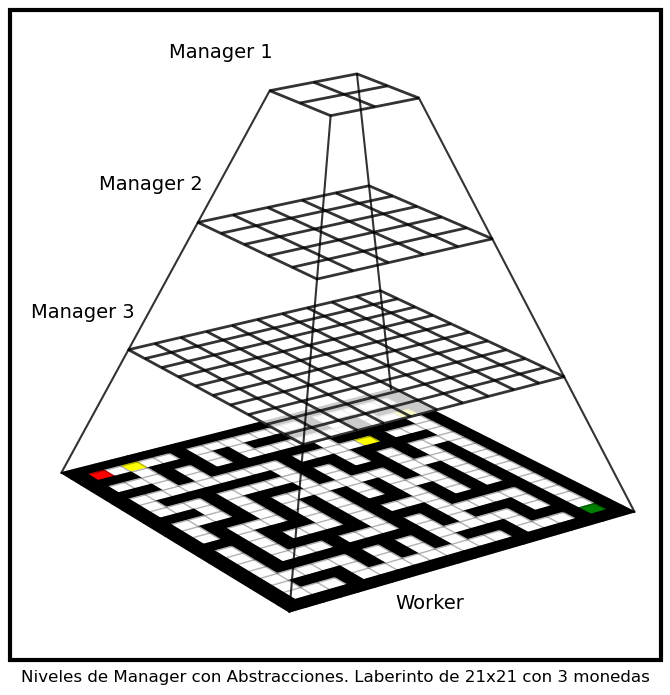
\includegraphics[width=0.7\columnwidth]{abstractions.png}
    \caption{Abstracciones y Niveles de Manager. Cuadros marcados: salida (verde), monedas (amarillo) y entrada (rojo) \label{fig:feudal-abstract}}
\end{figure}

A pesar de que este método se presenta prometedor, los resultados obtenidos no son aceptables (Fig \ref{fig:q-orig-results}). Para el 
problema base de navegación sin tareas intermedias, el algoritmo ha fallado en alcanzar el objetivo reiteradamente. Se destaca la falta
de obediencia por parte del worker que deriva en una mejora en el número de pasos y recompensa. No obstante, esto indica que el problema 
se encuentra en los \textit{managers} y sus órdenes. 

\begin{figure}[H]
    \centering
    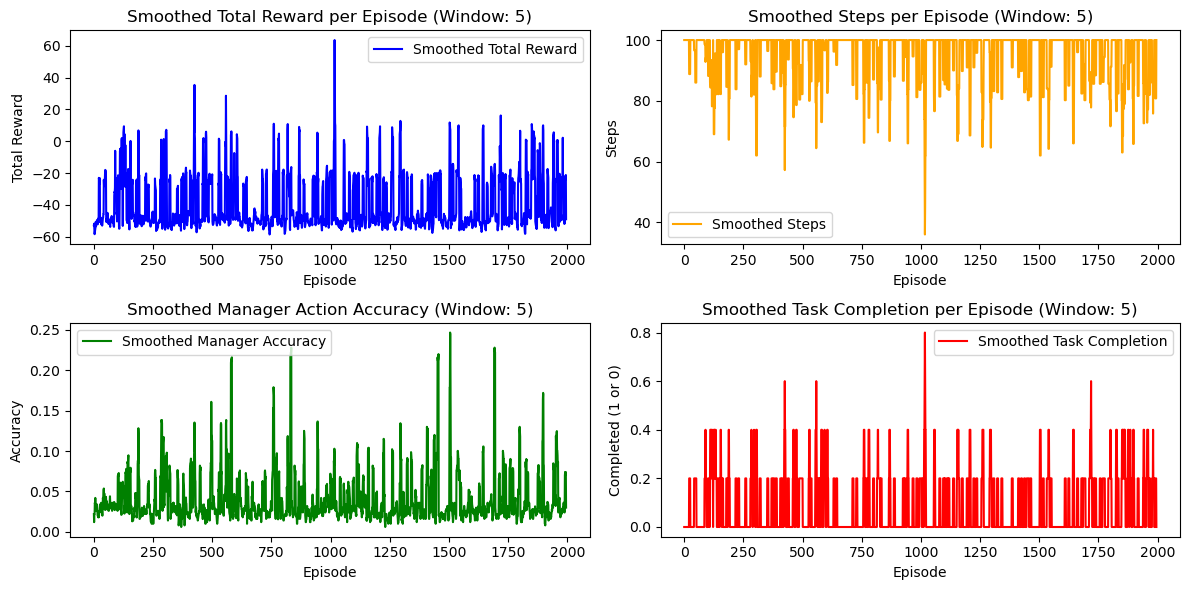
\includegraphics[width=0.9\columnwidth]{q-original-results.png}
    \caption{Feudal Q-Learning con 0 monedas.\label{fig:q-orig-results}}
\end{figure}

Tras un análisis de los resultados, se ha detectado un problema de representación que no se tenía en el experimento original. El laberinto contiene 
una gran cantidad de caminos sin salida y cerrados. En estos casos, los \textit{managers} no tienen percepción de las paredes y su representación puede incluir
intersecciones entre varias zonas paralelas. Este problema deriva en órdenes inválidas por parte de los \textit{manager} que desorientan al \textit{worker}. 

\subsection{Experimento: Feudal Q-Learning Modificado}

Debido a la disipación de las paredes que se experimentaba al realizar las abstracciones del mapa de estados a medida que se disminuía
el nivel del gerente, el aprendizaje resultaba altamente perjudicado, llegando a transmitirse órdenes imposibles de realizar debido a la
naturaleza cerrada del mapa del problema.

Para enfrentar dicha adversidad se probó a disminuir el número de gerentes/subgerentes, limitándose al uso del gerente de menor nivel
de abstracción; aquel que veía el mapa de estados en la escala original. Por lo tanto, se realizó una disminución de agentes para 
quedarse con únicamente 2: un gerente encargado de determinar la siguiente zona destino y otro agente encargado en navegar hasta 
dicha posición de interés. Dicha estructura contaba con las mismas limitaciones y políticas de recompensa definidas para el proceso anterior.

Para facilitar el arranque y el uso del mánager desde el principio, se facilitaba al mánager una pista de la localización de las monedas que 
debían ser recogidas para que guiara al trabajador (\textit{worker}) hacia dichas zonas sin necesidad de un proceso inicial donde las directrices del
manager podían ser “ignoradas” debido a su aleatoriedad. 

El trabajador a su vez realizaba un proceso de exploración que se veía recompensado cuando alcanzaba el punto objetivo determinado por el mánager.
Mediante estas exploraciones, iba creando sus caminos o matrices Q que iba actualizando y afinando con el fin de encontrar el camino óptimo a
partir de las recompensas obtenidas por obedecer al mánager.

En cuanto al proceso de aprendizaje, se incluyeron diferentes implementaciones para ver la influencia que estas variaciones o perturbaciones
tenían en el proceso de aprendizaje del super-agente. Las perturbaciones más comunes consistían en limitar el conocimiento que tenía el 
teacher (dándole solo el conocimiento de la solución empezando desde las coordenadas (1,1) o el conocimiento completo) o variando la posición
de comienzo del agente.

En cuento a los resultados que se obtuvieron sin ayudas externas, el proceso de aprendizaje era más lento al tener que explorar muchos estados y
 no contar con una ayuda externa en caso de caer en bucles debido a los estrechos caminos que componían el mapa (\ref{fig:maze-example}). Debido
  a este desconocimiento y falta de ayuda, las primeras iteraciones oscilaban en refuerzos negativos en su mayoría debido al proceso de exploración
   y explotación de conocimientos inciertos en dichas iteraciones. 

\begin{figure}[H]
    \centering
    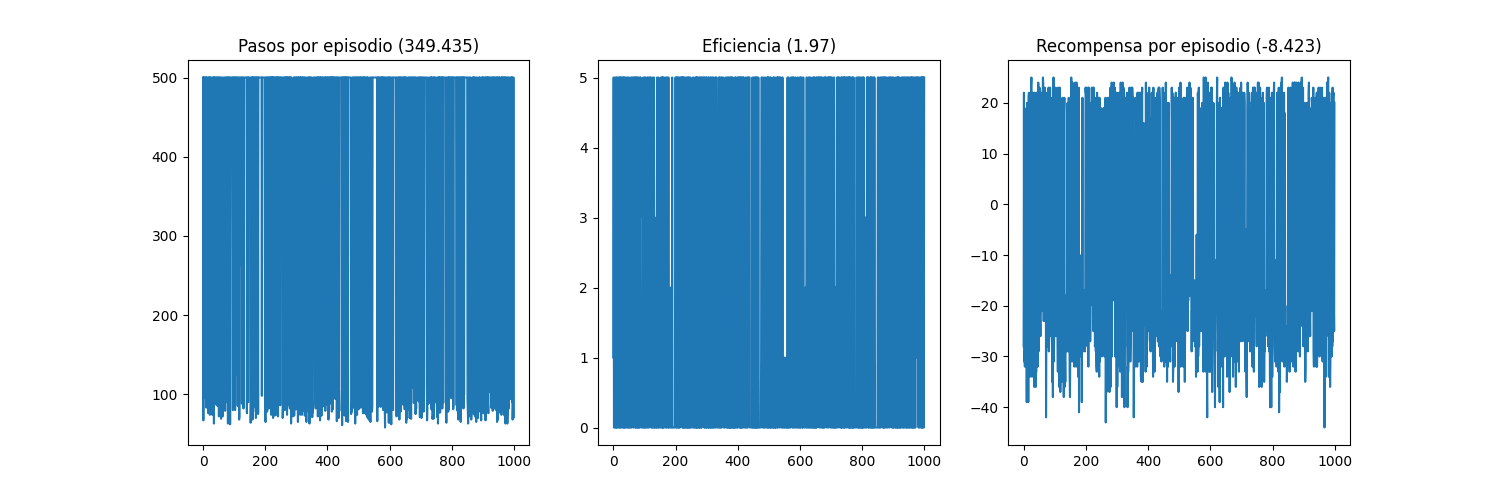
\includegraphics[width=0.9\columnwidth]{sin_ayuda_externa.png}
    \caption{Primeras 1000 iteraciones sin ayuda (16x16)\label{fig:FuN1}}
\end{figure}

Sin embargo, la influencia de un teacher con conocimiento de un solo camino ante el que siempre tenía la solución óptima suponía una gran diferencia.
 Mediante esta ayuda, el worker era capaz de afinar mejor la ruta a seguir y por lo tanto se vio un incremento en la cantidad de refuerzo medio que 
 se obtenían, pasando este a ser un valor positivo.

Aun así, al no contener información explotable desde todas las zonas del mapa de estados, se observaban procesos de oscilaciones también en los momentos
 en los que se partía de zonas inexploradas. Esto se debía a que el agente tenía que lograr llegar hasta el punto más cercano de donde tenía opción 
 de explotar conocimiento útil para poder obtener una ayuda, lo que lo ponía en similar situación que cuando no contaba con ayuda externa.

\begin{figure}[H]
    \centering
    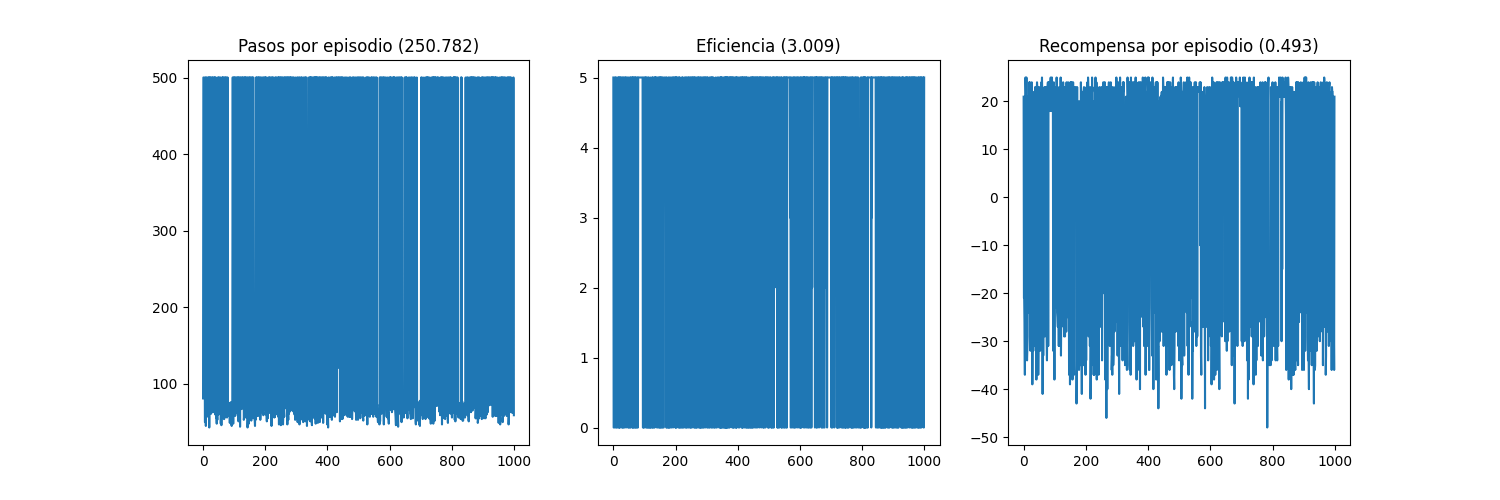
\includegraphics[width=0.9\columnwidth]{ayuda_externa_1path.png}
    \caption{Primeras 1000 iteraciones con ayuda simple (16x16)\label{fig:FuN2}}
    
\end{figure}

La máxima mejora del arranque inicial se logró mediante la introducción de rutas desde 3 zonas diferentes del mapa. Al depender del azar, estas
 rutas podrían aportar información redundante al tener inicios en lugares aleatorios del mapa, englobaban una mayor cantidad de estados, ofreciendo
  información explotable y útil en una subsección mayor del mapa. Debido a esto, la explotación del conocimiento y el reajuste ante un paso de 
  exploración indeseado eran corregidos lo que llevaba a evitar bucles o episodios perdidos.\footnote{\textsuperscript{}Situaciones en las que, 
  debido a entrar en un callejón, se realizaban pasos hasta llegar al límite de estos por episodio.}

\begin{figure}[H]
    \centering
    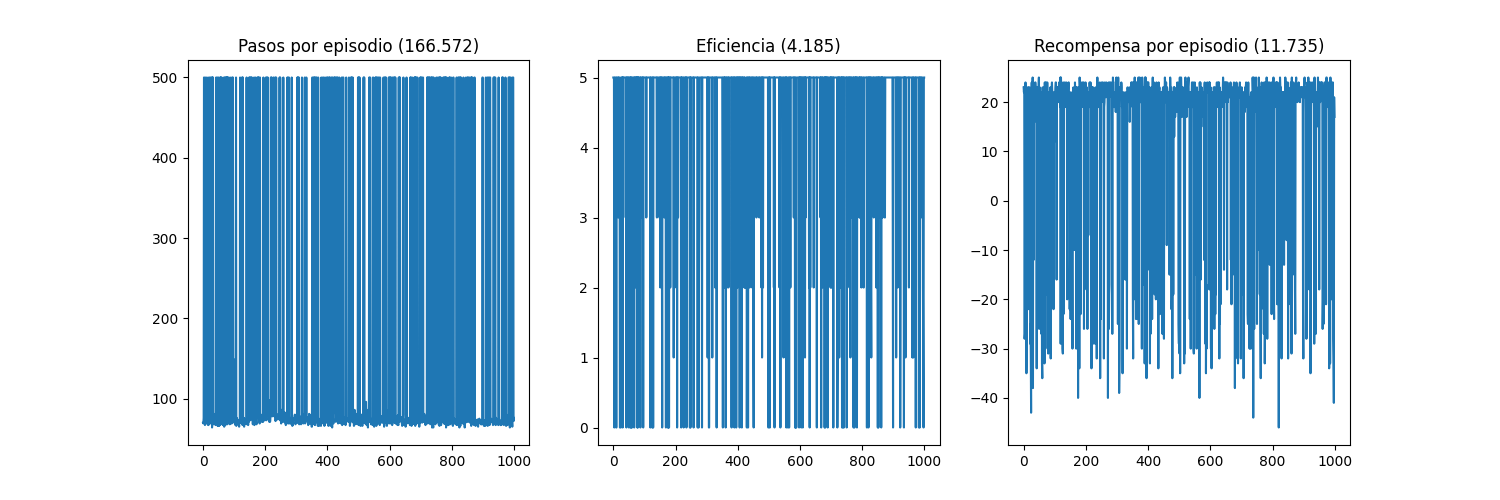
\includegraphics[width=0.9\columnwidth]{ayuda_externa_3paths.png}
    \caption{Primeras 1000 iteraciones con ayuda compleja (16x16)\label{fig:FuN3}}
\end{figure}

En conclusión, esta nueva estructura feudal, de un noble (\textit{mánager}) y un subordinado (\textit{worker}), supuso una mejora en comparación con el nivel anterior debida a la simplicidad y mayor énfasis en las limitaciones del mapa de estados que permitía definir. Mediante los experimentos que se realizaron se observó una mejora tanto en el proceso de aprendizaje como en la capacidad de llegar a soluciones en mapas de 20x20 tras 9000 iteraciones en caso de no incluir la ayuda externa o 1000 iteraciones cuando se le facilitaba el conocimiento explotable en 3 rutas. 

\begin{figure}[H]
    \centering
    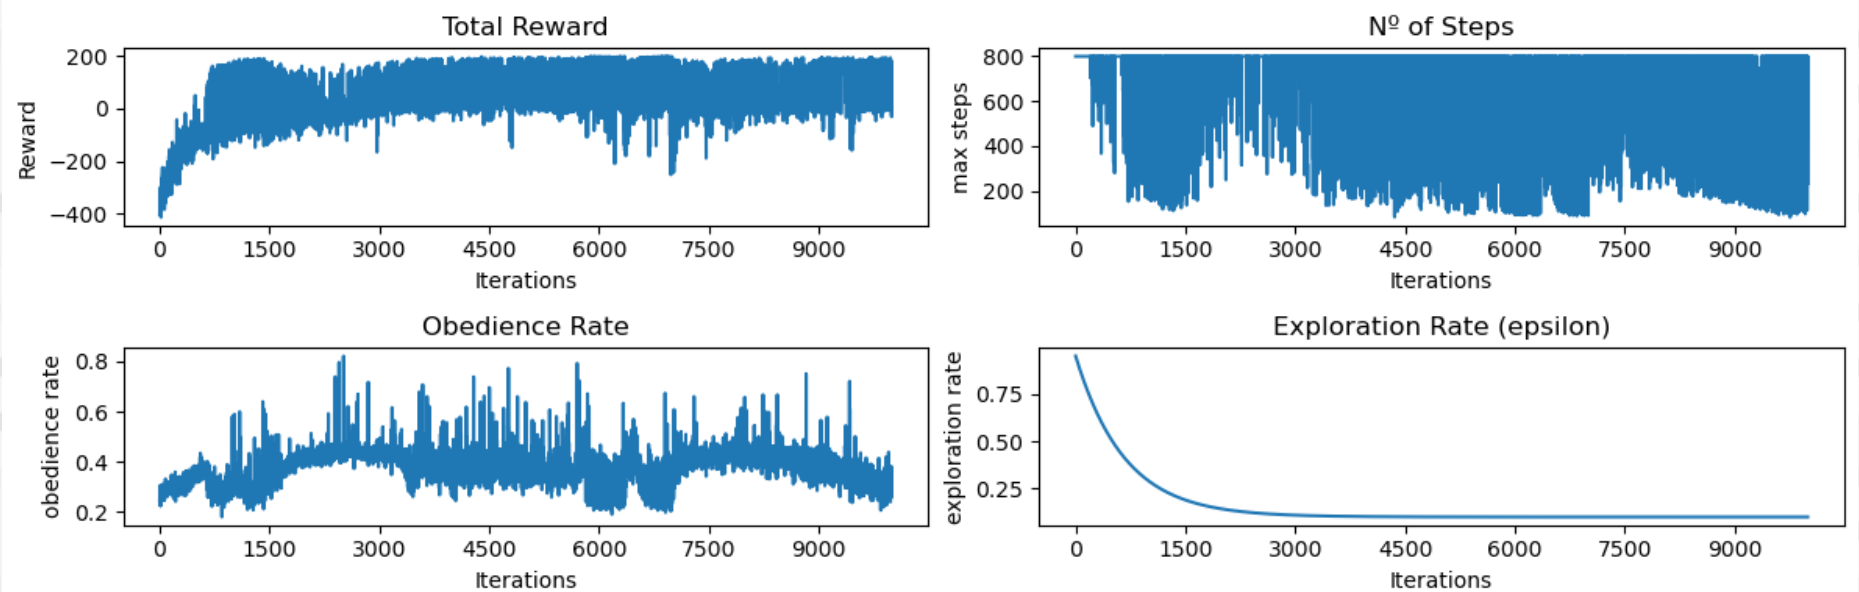
\includegraphics[width=0.9\columnwidth]{QL_resumen_final.png}
    \caption{Resultados tras 9000 iteraciones (20x20)}
    \label{fig:FuN1}
\end{figure}

\subsection{Experimento: FeUdal Networks (FUN)}

Otra técnica empleada de aprendizaje por refuerzo feudal son las FeUdal Networks (\textit{FuN}), basadas en LSTMs. Se creó una adaptación de este tipo de red para que pudiera funcionar en el dominio tratado, y se establecieron y probaron distintos refuerzos que proporcionar a la red, evaluando su efectividad a la hora de encontrar soluciones.

La primera versión del modelo FuN, emplea una función de refuerzo muy similar a la usada durante el Q-learning, en donde se da un refuerzo positivo por alcanzar los objetivos y se dan refuerzos negativos a medida que transcurre el tiempo sin alcanzar un objetivo. 
Esta primera versión no produjo resultados demasiado positivos, el modelo a veces lograba completar el laberinto, pero era común que se quedara atascado y que la pérdida no disminuyera. 
Todos los modelos probados en esta sección se han entrenado durante 500 épocas, con un límite de 2000 acciones por época (si en esas iteraciones no logra resolver el laberinto, 
se reinicia) y para comprobar si el modelo aprende correctamente se analizó si la pérdida disminuía a lo largo del tiempo. Se puede observar que no es el caso en la siguiente gráfica, donde el modelo aprende al principio y luego alcanza un punto estable.

\begin{figure}[H]
    \centering
    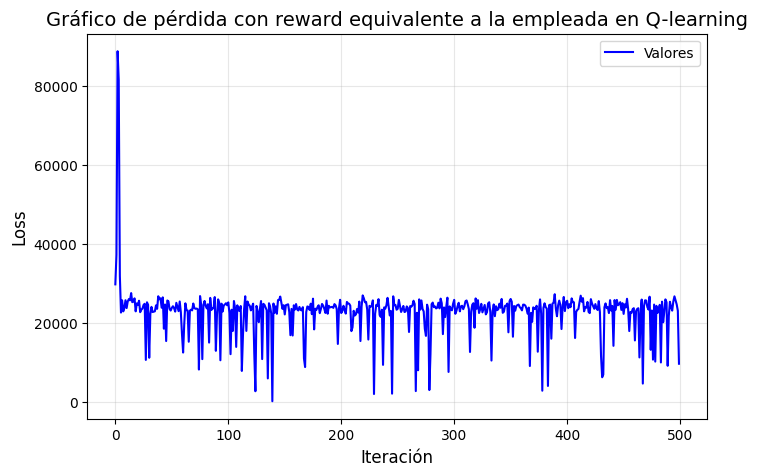
\includegraphics[width=0.9\columnwidth]{FuN_1.png}
    \caption{Pérdida de la primera versión.\label{fig:FuN6}}
\end{figure}

En la segunda versión, y para intentar mejorar la precisión del modelo, se añadió otra regla que penalizaba al modelo cuanto más lejos estuviera del objetivo definido por el mánager, para lo que se empleó la distancia de Manhattan. Esta nueva versión 
produjo resultados más inestables, donde no se llega a apreciar una auténtica mejora del modelo a lo largo del tiempo; los resultados se comparan con los de la versión anterior en la siguiente gráfica. Hay que tener en cuenta que la pérdida no está
en la misma escala entre las dos versiones, y lo importante que se debe observar es una disminución de esta a lo largo del tiempo, lo que indica que el modelo está aprendiendo, independientemente de la escala real de la pérdida. En la primera versión se 
penalizaba menos al modelo y por eso parece que tiene una pérdida menor, pero no quiere decir que sea mejor.

\begin{figure}[H]
    \centering
    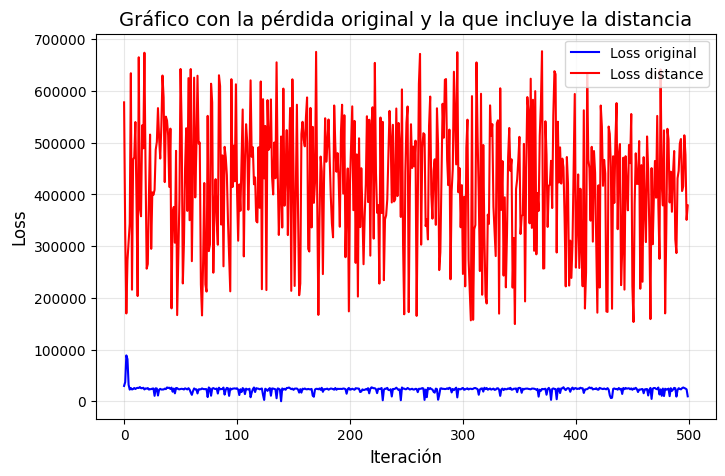
\includegraphics[width=0.9\columnwidth]{FuN_2.png}
    \caption{Pérdida de las dos primeras versiones.\label{fig:FuN4}}
\end{figure}

Se comprueba que no mejora demasiado a lo largo del tiempo, y los valores son más inestables, lo que no es necesariamente algo negativo, pero tampoco parece estar ayudando mucho al modelo.

Como tercera versión de este método, se añadió una recompensa por explorar estados nuevos y un castigo por repetir estados, lo que resultó en un nuevo modelo que, si bien sí que parece que aprenda, sigue sin producir soluciones mejores que los otros métodos. Es posible que si se entrenara durante el 
tiempo suficiente, y modificando los parámetros de las recompensas hasta alcanzar los mejores valores, se obtuvieran resultados similares e incluso mejores que los proporcionados por los otros métodos, pero requeriría una gran carga computacional.

Los resultados de esta versión, comparados con las otras dos, son los siguientes.
\begin{figure}[H]
    \centering
    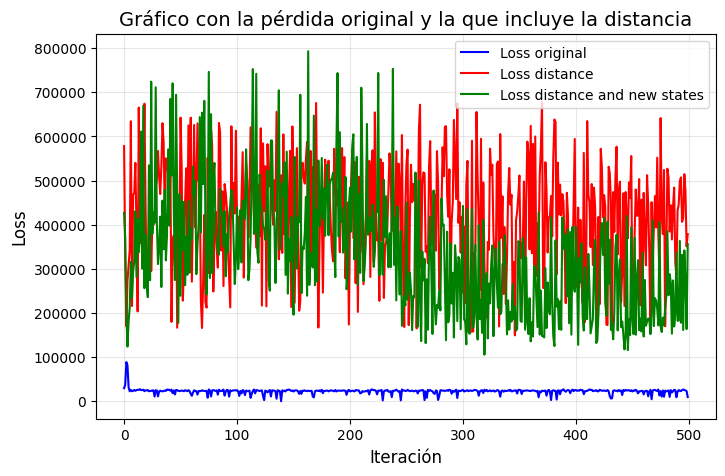
\includegraphics[width=0.9\columnwidth]{FuN_3.png}
    \caption{Pérdida de todas versiones.\label{fig:FuN5}}
\end{figure}

\section{Conclusiones}
En base al trabajo realizado, se puede concluir que las técnicas de aprendizaje por refuerzo jerárquico, específicamente el Aprendizaje por Refuerzo Feudal, añaden cierto valor añadido en aquellos problemas que cuentan con un fin complejo que se puede presentar como una suma de tareas a tratar de forma paralela y ordenada; en otras palabras, de forma jerárquica. Este sistema permite determinar agentes para cada nivel de abstracción estrictamente necesaria para la tarea, abstrayendo la decisión de problemas e inconvenientes pertenecientes a otras subtareas del problema.

Por el otro lado, se ha podido observar la influencia de la sobre-división de las tareas. Al dividir una tarea en demasiados niveles de abstracción, se realizaba una sobre-abstracción del espacio, lo que llevaba a tomar decisiones sin la información necesaria para dicha labor. En el caso del estudio realizado, dicho problema se ve bien representado en el caso de la selección de los destinos a navegar, donde debido a la excesiva abstracción del mapa de estados, se perdía la información espacial de las paredes. 

Debido a ello, se estima que, aunque dicha decisión se tome como abstraible en otras investigaciones, la naturaleza cerrada en cuestiones de navegación del problema tratado anulaba dicha característica.


\bibliography{aaai24}

\end{document}


